\chapter{Pipeline parallelism for Javascript} \label{chapter4}

%\chapter{A framework for parallel web applications}
 % \section{Fluxions}

% \chapter{Fluxion}

%   \section{Fluxionnal Compiler}
%     \comment{Some parts of this are already written in the first paper. It needs a lot additional explanations and rewritting}
%     \subsection{Identification}
%       \subsubsection{Continuation and listeners}
%       \subsubsection{Dues}
%     \subsection{Isolation}
%       \subsubsection{Scope identification}
%         \comment{Scope leaking}
%       \subsubsection{Execution and variable propagation}
%     \subsection{distribution}

%   \section{Fluxionnal execution model}
%     \comment{Everything here is already written in the first paper  : flx-paper. It only needs to be rewritten}
%     \subsection{Fluxion encapsulation}
%       \subsubsection{Execution}
%       \subsubsection{Name}
%       \subsubsection{Memory}
%     \subsection{Messaging system}

% \chapter{Evaluation}
%   \section{Due compiler}
%   \section{Fluxionnal compiler}
%   \section{Fluxionnal execution model}


The conclusion of the state of the art is that no platform allows to follow a project from the early beginning to the maturation of the project.
Indeed, no platform can provide alternatively productivity and efficiency.
All the platform tends to focus on a static compromise between these two goals, and therefore, are useful only at a precise point in the project.
They either grow useless, or are too complicated to begin with.

This chapter presents the solution developped in this thesis.
A platform to follow web application projects from the early beginning until the maturation of the project.

To support this evolution, it support a continuous developpement.

\section{Seamless Development} \label{chapter3:objectives}
\nt{TODO title not clear enough}


\begin{center}
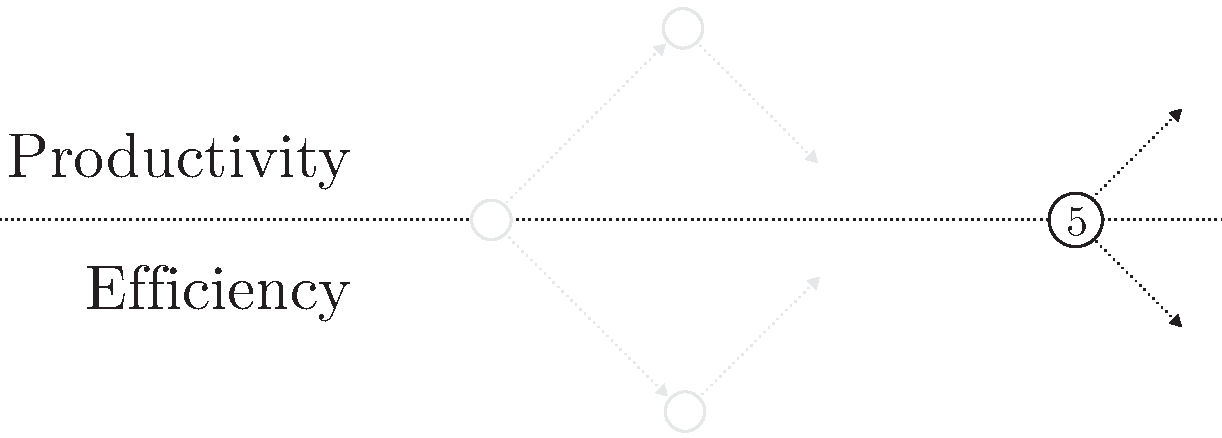
\includegraphics[width=0.6\textwidth]{../ressources/state-of-the-art-5.pdf}
\end{center}

% The objective of this thesis is to find a reconciliation of the two goals, by finding an equivalence between two approaches with different goals, in the case of streaming web applications.

The section \ref{chapter3:software-maintainability} shows that modularity and functional programming, especially higher-order programming and lazy evaluation, are the best organization to improve maintainability of an application.
This organization is best supported by a functional approach.
Indeed, higher-order programming improves readability and maintainability.
However, higher-order programming, and modular programming in general, requires the use of a global memory store.

The section \ref{chapter3:software-performance} shows that to attain scalability, an application needs to be organized to distribute its memory store into independent silos to provide isolation and immutability. Leading to multiply the exclusive accesses.
Still, many works provide this global memory store interface to developers, because it is the best way to support the modularity advocated in section \ref{chapter3:software-design}.
This incompatibility between these two organization, and their goals is responsible for the shifts operated during the life of an application.
Huge developing efforts are made to translate manually from one organization into the other, and to maintain the implementation despites its unmaintainable nature.
% when the most pressing need shift from maintainability to performance, or vice versa.

In section \ref{chapter3:objectives}, we show different tentatives to reconciles the two organizations.
Most are satisfactory for specific domains, such as the high-performance computing.
It is profitable, as the expected speedup of developing an application with an adapted programming model compensates the huge development effort.
%  where it is accepted to spend long time developing an application to use thousands of accelerators to compute heavy calculation, because the expected speedup is profitable, compared to develop an application for all these thousands accelerators.
However, none are satisfactory in the case of web applications because the need for performance is always uncertain.
The development effort is not required at the beginning, hence its cost cannot be justified.
It is only when the audience increases, often with the revenue, that the cost for the development effort can be justified.
This situation illustrate the need for a programming model reconciling the two concerns, of maintainability and performance.
% Indeed, they all are too specific, and require too much from the developer to be accepted at a large scale.

% \comment{Here a table summarizing the different approaches, and the sweet spot.}

Our objectives is to provide seamless development.
3.1 shows that modularity is not scalable but needed.
But compilation can help to get scalable.
3.2 shows that parallelism is not maintainable (no Higher-Order Programming, no lazy evaluation, so no good glue between modules)
But good developers can maintain double representation.
With help from an equivalence or a \textit{compiler} most developers could develop using this double representation, and seamlessly achieving parallelism and maintainability.

\begin{table}
\begin{tabular}{l|l|l|l}
             & Maintainability         & Performance           & Both\\\hline
General      & Functional Programming  & Message-passing       & Loop parallelization\\
Web          & Javascript              & Pipeline architecture & ø
\end{tabular}
\caption{Summary of the state of the art}
\label{tab:chapter3:objectives:summary}
\end{table}

\nt{integrate these paragraphs after the next section}
Our objectives is to find an equivalence between these two organization, specifically for the case of web applications.
To do so, we focus on the Javascript programming language, and specifically, the node.js interpreter.
\nt{TODO not clear}
As explained in the end of chapter \ref{chapter2}, the execution model of Javascript is similar to a pipeline.
We intend to split a node.js application into a parallel pipeline of stages.

The contribution of this thesis is organized in two chapters, as illustrated in figure \ref{fig:chapter3:objectives:roadmap}.
In chapter \ref{chapter4} I present the extraction of a pipeline of operations from a Javascript application.
I show that such pipeline is similar to the one exposed by Promises, and I propose a simpler alternative to the latter called Dues.
However, these operations still require a global memory for coordination so they are not executed in parallel.
In chapter \ref{chapter5}, we present the isolation of the operations into isolated containers called Fluxions. 

\begin{figure}[h!]
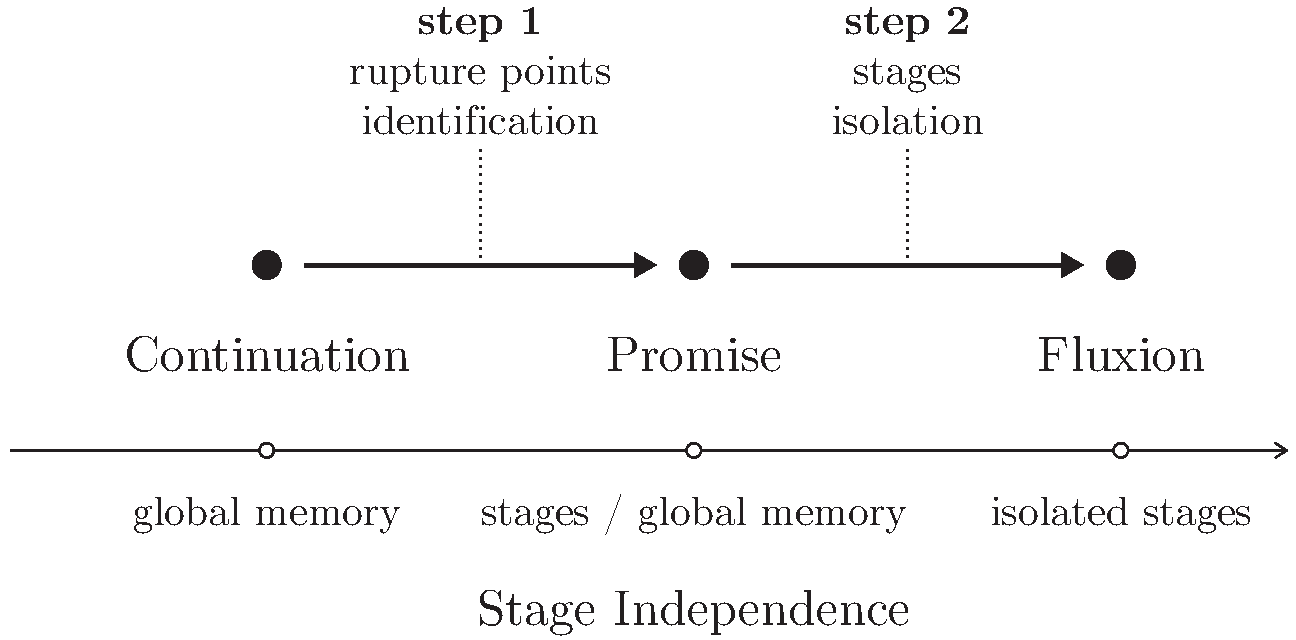
\includegraphics[width=1\textwidth]{../ressources/roadmap.pdf}
\caption{Roadmap for this work}
\label{fig:chapter3:objectives:roadmap}
\end{figure}

\begin{center}
\rule{3cm}{0.4pt}
need integration
\rule{3cm}{0.4pt}
\end{center}

We show that there is no languages that features higher-order functions to improve modularity, a common memory store easy to develop with, but at the same time provides scalable concurrency.

We aim at filling this gap, and for a concrete example, focus our work on the Javascript programing language.
Indeed, Javascript features higher-order functions, is highly-used in concurrent context, but lacks scalable concurrency.








\subsection{Equivalence}

\subsubsection{Rupture Point}

The execution of the pipeline architecture is well delimited in isolated stages.
Each stage has its own thread of execution, and is independent from the others.
On the contrary, the code of the event-loop is linear because of the continuation passing style and the common memory store.
% The message passing linking the callbacks is transparently handled by the event-loop.
However, the execution of the different callbacks are as distinct as the execution of the different stages of a pipeline.
The call stacks of two callbacks are distincts.
Therefore, an asynchronous function call represents the rupture between two call stacks.
It is a rupture point, and is equivalent to a data stream between two stages in the pipeline architecture.

Both the pipeline architecture and the event-loop present these rupture points.
The detection of rupture points allows to map a pipeline architecture onto the implementation following the event-loop model.
To allow the transformation from one to the other, this thesis studies the possibility to detect rupture points, and to distribute the global memory into the parts defined by these rupture points.
The detection of rupture points is addressed in chapter \ref{chapter4}.

\subsubsection{Invariance}

% This transformation is important on two points.
% The conservation of the invariance.
% The equivalence between the coordinations.

The transformation should preserve the invariance as expressed by the developer to assure the correctness of the execution.
The partial ordering of events in a system, by opposition to total ordering, is sufficient to assure this correctness.
% This result was used by Lamport to prove the correctness of distributed systems.
The global memory is a way to assure the total ordering of events, and the message passing coordination is a way to assure partial ordering of events.
Therefore, to assure the correctness of the execution of a system, the state coordination with a global memory is equivalent to message passing coordination.
And it is possible, at least for some rupture points, to transform the global memory coordination into message passing while conserving the correctness of execution.

In order to preserve the invariance assured by the event-loop model after the transformation, each stage of the pipeline needs to have an exclusive access to memory.
The global memory needs not to be split into parts and distributed into each of the stages.
To assure the missing coordinations assured by the shared memory between the stages, the transformation should provide equivalent coordination with message passing.
The isolation and replacement of the global memory is fully address in chapter \ref{chapter5}

% The invariance holds for the whole memory during the execution of each callback.
% As I explained in the previous section, this invariance is required to allow the concurrent execution of the different tasks.
% On the other hand, the invariance is explicit in the pipeline architecture, as all the stages have isolated memories.
% The coordination between these isolated process is made explicit by the developer through message passing.

% I argue that the state coordination between the callbacks requireing a global memory could be replaced by the message passing coordination used manually in the pipeline architecture.
% I argue that not all applications need concurrent access on the state, and therefore, need a shared memory.
% % Specifically, I argue that each state region remains roughly local to a stage during its modification.
% \nt{TODO review that, I don't know how to formulate these paragraphs. Identify the state and the data in the global memory.}

% \subsubsection{Transformation}

% This equivalence should allow the transformation of an event loop into several parallel processes communicating by messages.
% In this thesis, I study the static transformation of a program, but the equivalence should also hold for a dynamic transformation.
% I present the analyzis tools I developed to identify the state and the data from the global memory.

% # Explanation of the concept

## Turn-based programming.







(see presentation on Dues)
-> single-thread, no wait, no block and so on
Shared heap -> no mutex, no synchronization, so it is good scalability


Turn-based programming is an event-loop.
It is the execution of queued events one after the other.
An event is the association of a callback and a message.
The callback is a small Javascript Program, designed to process the message.
During its turn, the callback executes, and can queue events : that is register callback to be executed during a next turn.
TODO what I mean exactly by queue events ? -> the distinction between the asynchronous operation, and the resulting event.

## Pipeline

So a callback sends messages to other callbacks.
-> It is exactly like a pipeline.
However, all the callbacks share the same heap.
So it is not possible to distribute the different callbacks without synchronization of this heap, or splitting the heap for each callback.
TODO state VERY clearly this problem, it is at the core of my thesis.

So, how to split the heap so that each callback has its own exclusive heap ?

## Propagation of variables.

Javascript is lexically scoped, therefore we can identify the scope of variable statically.
(At the exception of eval and with : with is forbidden from strict mode, so that is not a bigdeal, howether, eval is sometimes used in smart ways, but most of the time it is monomorphic (I don't exactly know what that means, I heard from Floreat, it must be something related to PL community)).

### Scope identification

The compiler identifies the variables shared by multiple callbacks from their scope.
TODO explain this in depth.
Function scope, closures, and so on ...

### Scope leaking

Javascript uses a pass-by-sharing paradigm.
That means that sometimes the argument of a call are passed by value, sometimes by reference (atomic data type (number, string, bool) -> by value, complex data type (objects) -> by reference).
That means that the modification of a local variable can affect variable in seemingly unrelated scopes.
It seems that the points-to analysis is what is used to find stuffs like that (side-effects ?).

### Propagation of execution and variables

The execution progress downstream, following the message stream.
TODO state very clearly this proposition, it is the second core of my thesis (and I love the idea, it relates directly to reality, graivity, and the fabric of the universe <3).

Because the propagation of the modification is not instantaneous, going back upstream is like going backward in time : it is impossible.
Therefore, a variable cannot be read upstream a write.
And it cannot be write downstream either.

In other words, only one callback can write on a variable -> seems obvious from previous sections.


In promises, because the heap is not shared, things are less restrictive.
Multiple stages can read and write the same variable, because the propagation of modification is instantaneous, due to the shared heap.